This paper emphasizes the necessity of using textual information 
to qualitatively fit the edge weights $w^*$ for the \textit{directed weighted graph} $G^*$ that is defined in Figure \ref{fig:def}. 
One can simply consider a co-citation pattern between the articles of WTO agreements as a a regulatory system of WTO DSB, however,
it simply allocates a huge edge weight for frequently cited articles and fails to explain how articles interact to achieve main principles of WTO as exemplified in Figure \ref{fig:market-aceess_directed}.

This failure is mainly due to the insufficient information in co-citation matrix. Members tend to cite the articles of 
the WTO agreements based on the complex characteristics of 
the trade policy that led to the dispute, however, co-citation pattern omits this prior information.

To emphasize the importance of using textual information, I prepared two differeent matrices $W_{\text{co-cites}}$ and $W_{\text{text}}$ that is following the definition of \textit{edge weight matrix} $W$ in Figure \ref{fig:def}.
$W_{\text{co-cites}}$ is calculated only using the co-citation pattern between articles of the WTO agreements as formally defined in Figure \ref{fig:def-illus-normal-co-cites}. 
$W_{\text{text}}$ is the one that is fitted using the textual information and the way how it's fitted will be introduced at the following body in this section.
Two Heatmaps visualized in Figure \ref{fig:heatmap:edgeweights:compare} shows how sparse the $W_{\text{co-cites}}$ is. This sparisty led to the insufficient information
to qualitatively maps the regulatory system of WTO DSB. In contrast with it, if we fit the \textit{edge weight matrix} $W$ using the textual information, we get more dense matrix as visualized in Figure\ref{subfig:adj_dense}.

% and visualized them as a heatmap in Figure \ref{fig:heatmap:edgeweights:compare}.
% $W_{\text{co-cites}}$ is an edge weight matrix that is calculated only using the co-citation pattern between articles without textual information. 

% We can compare two weight matrices of each network that maps the regulatory system of WTO DSB as a network of articles of WTO agreements in Figure \ref{fig:sparse_dense}.
% == HEATMAP MATRIX == 
\begin{figure}[ht]
    \begin{subfigure}[b]{0.49\textwidth}
        \centering{
            \resizebox{\textwidth*\real{\heatmap}}{\textwidth*\real{\heatmap} * \real{1}}{% This file was created by tikzplotlib v0.9.4.
\begin{tikzpicture}

\begin{axis}[
tick align=outside,
tick pos=left,
title={coo},
x grid style={white!69.0196078431373!black},
xmin=0, xmax=58,
xtick style={color=black},
y grid style={white!69.0196078431373!black},
ymin=0, ymax=58,
ytick style={color=black}
]
\addplot graphics [includegraphics cmd=\pgfimage,xmin=0, xmax=58, ymin=0, ymax=58] {coo-001.png};
\end{axis}

\end{tikzpicture}
}
            \caption{$W_{\text{co-cites}}$}
            \label{subfig:adj_sparse}
        }
    \end{subfigure}
    % \hfill
    % \pgfdeclareverticalshading{colormap}{0.2cm}{rgb(0.0pt)=(0,1,1); rgb(6cm)=(0.8784,0.6902,0.99998)}
    % \pgfuseshading{colormap}
    \hfill
    \begin{subfigure}[b]{0.49\textwidth}
        \centering{
            \resizebox{\textwidth*\real{\heatmap}}{\textwidth*\real{\heatmap} * \real{1}}{% This file was created by tikzplotlib v0.9.4.
\begin{tikzpicture}

\begin{axis}[
hide x axis,
hide y axis,
tick align=outside,
tick pos=left,
x grid style={white!69.0196078431373!black},
xmin=0, xmax=80,
xtick style={color=black},
y grid style={white!69.0196078431373!black},
ymin=0, ymax=80,
ytick style={color=black}
]
\addplot graphics [includegraphics cmd=\pgfimage,xmin=0, xmax=80, ymin=0, ymax=80] {coo_dense-002.png};
\end{axis}

\end{tikzpicture}
}
            \caption{$W_{\text{text}}$}
            \label{subfig:adj_dense}
        }
    \end{subfigure}
    \label{fig:sparse_dense}
    \vfill
    \centering{
        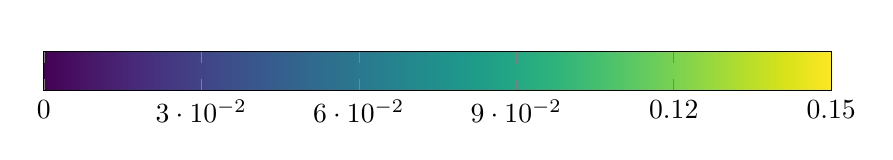
\begin{tikzpicture}
    \begin{axis}[
            hide axis,
            scale only axis,
            height=0pt,
            width=0pt,
            colormap/viridis,
            colorbar horizontal,
            point meta min=0,
            point meta max=0.15,
            colorbar style={
                    width=10cm,
                    height=0.5cm,
                    xtick={0,0.03,0.06,0.09,0.12,0.15}
                }]
        \addplot [draw=none] coordinates {(0,0)};
    \end{axis}
\end{tikzpicture}
    }
    \caption{\textbf{Heatmap of Two Different Edge Weight Matrices: }Above two subfigures visualizes two different \textit{edge weight matrices} $W_{\text{co-cites}}$ and $W_{\text{text}}$. One can check that $W_{\text{co-cites}}$ is sparser than $W_{\text{text}}$.}
    \label{fig:heatmap:edgeweights:compare}
\end{figure}


% % == DEF EXAMPLE == 
\begin{figure}[h]
    \begin{subfigure}[b]{1\textwidth}
        \[\text{Let } \delta^d_{ij} \text{ is defined to be } 1 \text{ if } \{(v_i, v_j) \mid v_i, v_j \in V \text{ and } i \neq j \} \subset c_{d \in D} \ \text{ else } 0\]
        \[\text{ where } V, D \text{ and } c_d \text{ is defined as in Figure \ref{fig:def:set-of-cited-articles}}. \]
        \[\text{Then let \textit{co-citation matrix} } M = (m_{ij}) \in \Bbb{N}^{|V| \times |V|} \text{ s.t. } m_{ij} = \sum_{d \in D}\sum_{i,j \in V}\delta^d_{ij}\]
        \caption{\textbf{Formal Definition of Co-citation Matrix}}
        \label{subfig:co-cites:def}
    \end{subfigure}
    \vfill
    \begin{subfigure}[b]{1\textwidth}
        \centering{
            % \begin{figure}[h]
%     \centering
    \begin{tikzpicture}
        \foreach \i in {\xMin,...,5} {
            \draw [black] (\i,4) -- (\i,9) node [below] at (\i,4) {};
        }
        \foreach \i in {4,...,9} {
            \draw [black] (\xMin,\i) -- (5,\i) node [left] at (\xMin,\i) {};
        }

        % \node [left] at (0,0.5) {\textbf{XXVIII}};
        % \node [left] at (0,1.5) {\textbf{XXVI:6}};
        % \node [left] at (0,2.5) {\textbf{XXIV:5(b)}};
        % \node [left] at (0,3.5) {\textbf{XXIV:12}};
        \node [left] at (0,4.5) {\textbf{\vdots}};
        \node [left] at (0,5.5) {\textbf{II:1}};
        \node [left] at (0,6.5) {\textbf{II}};
        \node [left] at (0,7.5) {\textbf{I:1}};
        \node [left] at (0,8.5) {\textbf{I}};

        % \node [left] at (8.8, 9.25) {\textbf{XXVIII}};
        % \node [left] at (7.8, 9.25) {\textbf{XXVI:6}};
        % \node [left] at (6.8, 9.25) {\textbf{XXIV:5(b)}};
        % \node [left] at (5.8, 9.25) {\textbf{XXIV:12}};
        \node [left] at (4.8, 9.25) {\textbf{\ldots}};
        \node [left] at (3.8, 9.25) {\textbf{II:1}};
        \node [left] at (2.8, 9.25) {\textbf{II}};
        \node [left] at (1.85, 9.25) {\textbf{I:1}};
        \node [left] at (0.7,9.25) {\textbf{I}};

        \node [left] at (0.7,8.5) {\textbf{0}};
        \node [left] at (1.7,8.5) {\textbf{3}};
        \node [left] at (2.8,8.5) {\textbf{7}};
        \node [left] at (3.8,8.5) {\textbf{2}};
        
        \node [left] at (0.7,7.5) {\textbf{3}};
        \node [left] at (1.7,7.5) {\textbf{0}};
        \node [left] at (2.8,7.5) {\textbf{3}};
        \node [left] at (3.8,7.5) {\textbf{4}};

        \node [left] at (0.7,6.5) {\textbf{7}};
        \node [left] at (1.7,6.5) {\textbf{3}};
        \node [left] at (2.8,6.5) {\textbf{0}};
        \node [left] at (3.8,6.5) {\textbf{4}};

        \node [left] at (0.7,5.5) {\textbf{2}};
        \node [left] at (1.7,5.5) {\textbf{4}};
        \node [left] at (2.8,5.5) {\textbf{4}};
        \node [left] at (3.8,5.5) {\textbf{0}};



        % \node [left] at (5.5,9.5) {\textbf{Embedding Dimension = $k$}};
        % \node [right, rotate=-90, font=\small] at (6.5,7) {\textbf{Max Sequence Length = $n$}};


    % \draw [step=1.0,blue, very thick] (0.5,0.5) grid (5.5,4.5);
    % \draw [very thick, brown, step=1.0cm,xshift=-0.5cm, yshift=-0.5cm] (0.5,0.5) grid +(5.5,4.5);
    \end{tikzpicture} 
%     \label{fig:visualize-co-cites}      
%     \caption{\textbf{Definition of Co-citation Matrix:} This paper defines co-citation matrix $C$ as a $\mid V \mid \times \mid V \mid$ matrix where each element $c_{ij}:= \text{Counts of } $ is count of all co-occurrence $  \text{ } s.t. \text{ } \forall i,j \in \mid V \mid$ } 
% \end{figure}

% This  dispute  concerns  the  Continued  Dumping 
            \caption{\textbf{Illustration of Co-citation Matrix}}
            \label{subfig:co-cites:illus}
        }
    \end{subfigure}
    \label{fig:def-illus-co-cites}      
    \caption{\textbf{Formal Definition and Illustration of Co-citation Matrix:} This paper defines co-citation matrix $M$ as subfigure $(a)$ and it is illustrated as subfigure $(b)$.} 
\end{figure}
\begin{figure}[t!]
    \begin{subfigure}[b]{1\textwidth}
        \[\text{For given $M$ defined in Figure \ref{subfig:co-cites:def},} \]
        \[\text{let \textit{normalized co-citation matrix} } N = (n_{ij}) \in \Bbb{R}^{|V| \times |V|} \text{ s.t. } n_{ij} = \frac{m_{ij}}{\sum_{j \in V}m_{ij}} \]
        \caption{\textbf{Formal Definition of Normalized Co-citation Matrix}}
        \label{subfig:co-cites:def:normal}
    \end{subfigure}
    \vfill
    \begin{subfigure}[b]{1\textwidth}
        \centering{
            % \begin{figure}[h]
%     \centering
    \begin{tikzpicture}
        \foreach \i in {\xMin,...,5} {
            \draw [black] (\i,4) -- (\i,9) node [below] at (\i,4) {};
        }
        \foreach \i in {4,...,9} {
            \draw [black] (\xMin,\i) -- (5,\i) node [left] at (\xMin,\i) {};
        }

        % \node [left] at (0,0.5) {\textbf{XXVIII}};
        % \node [left] at (0,1.5) {\textbf{XXVI:6}};
        % \node [left] at (0,2.5) {\textbf{XXIV:5(b)}};
        % \node [left] at (0,3.5) {\textbf{XXIV:12}};
        \node [left] at (0,4.5) {\textbf{\vdots}};
        \node [left] at (0,5.5) {\textbf{II:1}};
        \node [left] at (0,6.5) {\textbf{II}};
        \node [left] at (0,7.5) {\textbf{I:1}};
        \node [left] at (0,8.5) {\textbf{I}};

        % \node [left] at (8.8, 9.25) {\textbf{XXVIII}};
        % \node [left] at (7.8, 9.25) {\textbf{XXVI:6}};
        % \node [left] at (6.8, 9.25) {\textbf{XXIV:5(b)}};
        % \node [left] at (5.8, 9.25) {\textbf{XXIV:12}};
        \node [left] at (4.8, 9.25) {\textbf{\ldots}};
        \node [left] at (3.8, 9.25) {\textbf{II:1}};
        \node [left] at (2.8, 9.25) {\textbf{II}};
        \node [left] at (1.85, 9.25) {\textbf{I:1}};
        \node [left] at (0.7,9.25) {\textbf{I}};

        \node [left] at (0.7,8.5) {\textbf{0}};
        \node [left] at (2.1,8.5) {\textbf{0.053}};
        \node [left] at (3.1,8.5) {\textbf{0.125}};
        \node [left] at (4.1,8.5) {\textbf{0.035}};
        
        \node [left] at (1.1,7.5) {\textbf{0.040}};
        \node [left] at (1.8,7.5) {\textbf{0}};
        \node [left] at (3,7.5) {\textbf{0.04}};
        \node [left] at (4.1,7.5) {\textbf{0.054}};

        \node [left] at (1.1,6.5) {\textbf{0.114}};
        \node [left] at (2.1,6.5) {\textbf{0.049}};
        \node [left] at (2.8,6.5) {\textbf{0}};
        \node [left] at (4.1,6.5) {\textbf{0.065}};

        \node [left] at (1.1,5.5) {\textbf{0.032}};
        \node [left] at (2.1,5.5) {\textbf{0.065}};
        \node [left] at (3.1,5.5) {\textbf{0.065}};
        \node [left] at (3.7,5.5) {\textbf{0}};

        \draw[->, densely dotted, thin] (4.2,8.5) -- (6,8.5) node[right] {$\sum_{j \in V} n_{ij} = 1$};

        % \node [left] at (10,8.5) {-> \textbf{Embedding Dimension = $k$}};
        % \node [right, rotate=-90, font=\small] at (6.5,7) {\textbf{Max Sequence Length = $n$}};


    % \draw [step=1.0,blue, very thick] (0.5,0.5) grid (5.5,4.5);
    % \draw [very thick, brown, step=1.0cm,xshift=-0.5cm, yshift=-0.5cm] (0.5,0.5) grid +(5.5,4.5);
    \end{tikzpicture} 
%     \label{fig:visualize-co-cites}      
%     \caption{\textbf{Definition of Co-citation Matrix:} This paper defines co-citation matrix $C$ as a $\mid V \mid \times \mid V \mid$ matrix where each element $c_{ij}:= \text{Counts of } $ is count of all co-occurrence $  \text{ } s.t. \text{ } \forall i,j \in \mid V \mid$ } 
% \end{figure}

% This  dispute  concerns  the  Continued  Dumping 
            \caption{\textbf{Illustration of Noramlized Co-citation Matrix}}
            \label{subfig:co-cites:illus:normal}
        }
    \end{subfigure}
    \caption{\textbf{Formal Definition and Illustration of Normalized Co-citation Matrix:} This paper defines normalized co-citation matrix $N$ of $M$ as subfigure $(a)$ and it's illustrated as subfigure $(b)$ using the paper's dataset. Note that normalized co-citation matrix is no more \textit{symmetric}, $n_{ij} \neq n_{ji} \text{ } \forall i,j \in V$. This definition is prepared to fit the definition of co-citation matrix to that of $W$ as defined in Section \ref{subsec:def}.} 
    \label{fig:def-illus-normal-co-cites}
\end{figure}



% This paper will compare two different results that one uses textual information using deep learning and the other one
% uses the frequency of co-citation only after explaining how deep learning works to encompass the textual information.

% if a method 
% do not consider a way to encompass the information
% about the identiy of the trade policy at issue with 
% each article's regulatory content written in its own article text,
% it can only reflect how articles of WTO agreements are co-cited 
% together rather than reflecting how articles of WTO agreements 
% cooperates to regulate each charactersitic of complex trade policy that led to the dispute. 
